\section{Indledning}
Projektet omhandler behandling af lyd, objektorienteret programmering samt en brug af datakommunikation og softwareudvikling.

To bærbare computere skal kommunikere med hinanden ved hjælp af lyd, hvortil der blev udleveret 2 sæt mikrofoner og højtalere.
Der skal bruges DTMF-toner til kommunikationen. Disse har har været brugt i gamle telefoner til transmission af telefonnumre over telefonnettet. DTMF står for "Dual Tone Multiple Frequency", hvilket betyder at der ligger to toner oven i hinanden med forskellige frekvenser. Afspilles tone '1', vil dette eksempelvis indebære frekvenserne 697 Hz og 1209 Hz. \footnote{Digital Signal processing, kapitel 8.11}.

\begin{figure}[h]
\centering
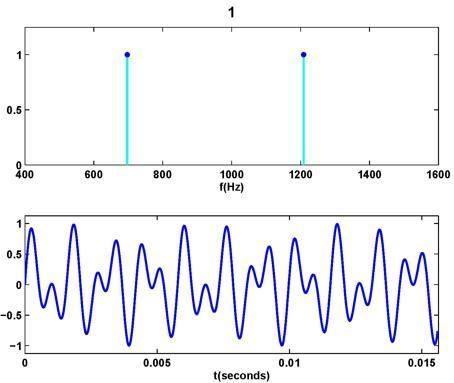
\includegraphics[scale=0.5]{Billeder/DTMF1.JPG}
\caption{DTMF-tone 1}
\label{fig:DTMF1}
\end{figure}

Projektet skal skrives i programmeringssproget C++, som er et objektorienteret sprog. Samtidigt skal softwarearkitekturen være lagdelt, eksempelvis ved et fysisk lag og et datalinklag.
Programmet der udvikles skal som krav udføre noget meningsfyldt, såsom en styring til en legetøjs bil, eller understøttelse af et multiplayer spil.